\documentclass{beamer}

\usepackage[utf8]{inputenc}
\usepackage[swedish]{babel}
\usepackage[lighttt]{lmodern}
\usepackage{graphicx}

\usetheme{CambridgeUS}
\title{Fossiloberoende bilflotta i Sverige år 2030}
\author[Andreas \and Daniel \and Magnus \and Niclas \and Robert]{Andreas Hagesjö \and Daniel Pettersson \and
Magnus Hagmar \and Niclas Ogeryd \and Robert Nyquist}

\begin{document}

\frame{\titlepage}

\begin{frame}
	\frametitle{Introduktion}
	\framesubtitle{Frågeställning}
	\begin{itemize}
		\item Aktuellt
		\item Regeringen
		\item Optimistisk framtid
		\item Tekniska utvecklingar
	\end{itemize}
\end{frame}

\begin{frame}
	\frametitle{Introduktion}
	\framesubtitle{Fossiloberoende?}
	\begin{itemize}
		\item Möjligt att köra utan fossila bränslen
		\item Inte ett måste
		\item Bränslesäkerhet
		\item Effektivitet
	\end{itemize}
\end{frame}

\begin{frame}
	\frametitle{Introduktion}
	\framesubtitle{Transportbränslen}
	\begin{itemize}
		\item El
			\begin{itemize}
				\item Kärnkraft, upphävt förbud
				\item Högre effektivitet
				\item Laddhybrider säljs idag
				\item Styrmedel, supermiljöbilspremie
			\end{itemize}
		\item Vätgas
			\begin{itemize}
				\item Produceras i små mängder
				\item Få tankstationer
				\item Dyrt
			\end{itemize}
		\item Biobränsle
			\begin{itemize}
				\item Tunga fordon kräver stor mängd energi
				\item Konvertera existerande diesel/bensinbilar
				\item Avdragsgill
				\item Ökad efterfrågan, land-grabbing, bränslesäkerhet
			\end{itemize}
	\end{itemize}
\end{frame}

\begin{frame}
	\frametitle{Metod}
	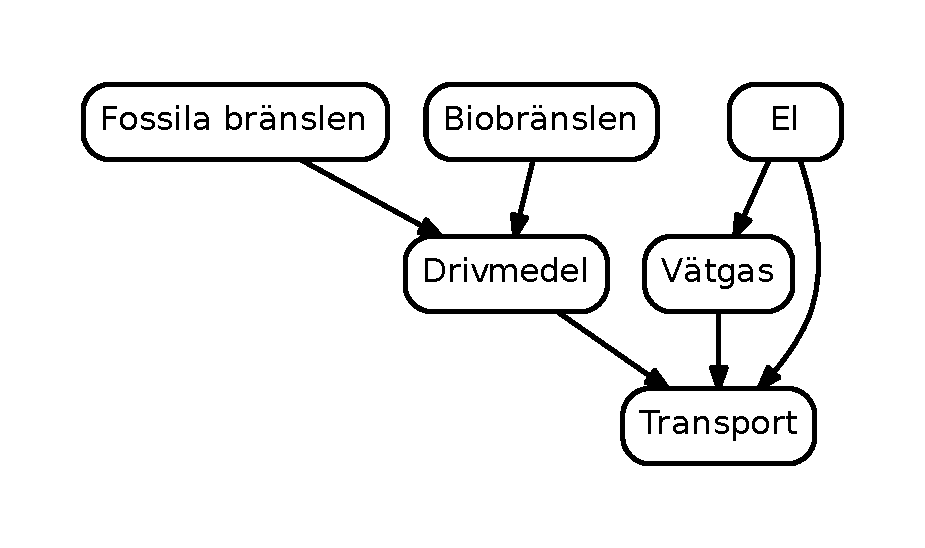
\includegraphics[scale=0.5]{../report2/diagram.pdf}
	\begin{itemize}
		\item Utgått från modell i tidigare uppgift
		\item Förenklad utan transmission och verkningsgrader
		\item Svårt att ta fram hypotes
		\item Korrekt resultat från algoritm
	\end{itemize}
\end{frame}

\begin{frame}
	\frametitle{Scenario 1}
	\framesubtitle{Bio och El}
	\begin{itemize}
		\item Kraftig ökning av biodrivmedel
		\item Fler elbilar
	\end{itemize}
\end{frame}

\begin{frame}
	\frametitle{Scenario 1}
	\framesubtitle{Bio och El}
	\begin{figure}[h!]
	\begin{center}
	\begin{tabular}{ | l | l | l | }
	\hline
						& Nu		& 2030 \\ \hline
	Fossil energi				& 94 TWh	& 22,2 TWh \\ \hline
	Biobränsle				& 11 TWh	& 60 TWh \\ \hline % 91% av energianvändningen
	El					& (Nästan) 0 TWh &  2,2 TWh \\ \hline % ~6% av bilenergianvändningen
	Total energianvändning		& 105 TWh	& 86 TWh \\ \hline
	Energianvändning av personbilar	& 50 TWh	& 35 TWh \\ \hline
	\end{tabular}
	\caption{Energianvändning i transportsektorn}
	\label{tab:scen1energi}
	\end{center}
	\end{figure}
\end{frame}

\begin{frame}
	\frametitle{Scenario 1}
	\framesubtitle{Bio och El}
	\begin{figure}[h!]
       \centering
       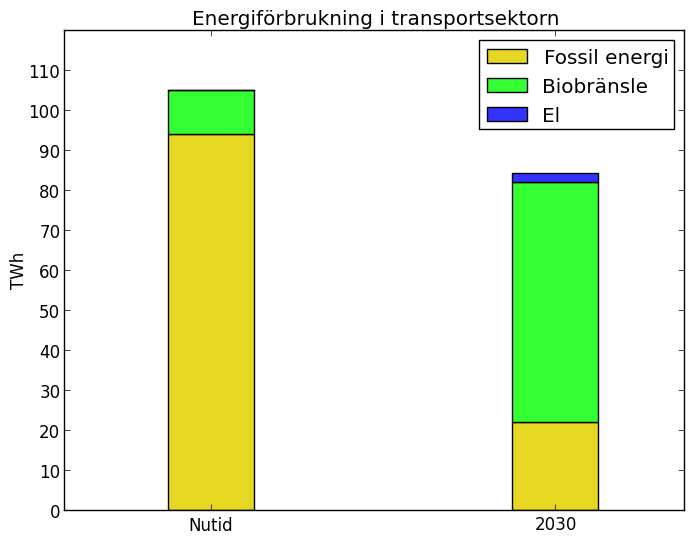
\includegraphics[scale=0.7]{scen1a1transport.png}
       \caption{Fördelning av energi i transportsektorn scenario 1 alternativ 1}
	\end{figure}
\end{frame}

\begin{frame}
	\frametitle{Scenario 2}
	\framesubtitle{Vätgas}
	\begin{itemize}
		\item 
	\end{itemize}
\end{frame}

\begin{frame}
	\frametitle{Diskussion}
	\framesubtitle{Bio och El}
	\begin{itemize}
		\item Ökad produktion av biomaterial
		\item Mer elproduktion
		\item Fordonsbyte - styrmedel
		\item Forskning och utveckling
	\end{itemize}
\end{frame}

\begin{frame}
	\frametitle{Diskussion}
	\framesubtitle{Bio och El - Alternativ 1}
	\begin{itemize}
		\item{''Flytta'' fossil och bio}
		\item{Öka bioproduktion}
		\item{Importera biodrivmedel?}
		\item{Ökad vind- och kärnkraft}
	\end{itemize}
\end{frame}

\begin{frame}
	\frametitle{Diskussion}
	\framesubtitle{Bio och El - Alternativ 1
	\begin{figure}[h!]
       \centering
       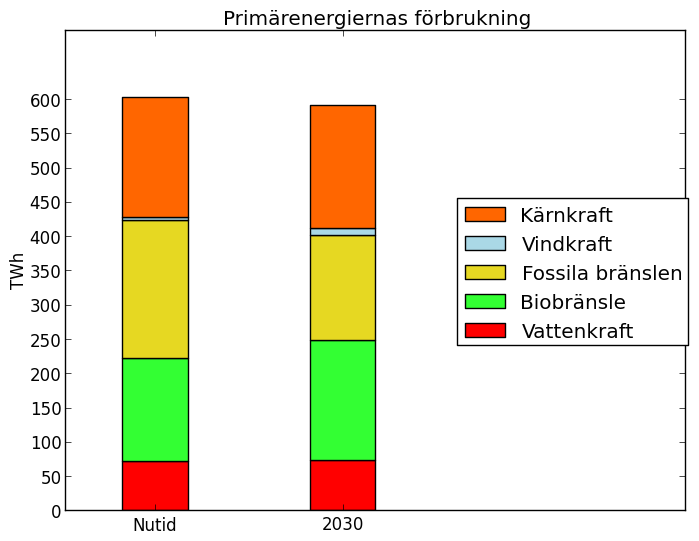
\includegraphics[scale=0.7]{scen1a1energidiagram.png}
       \caption{Primärenergiernas energiförbrukning för scenario 1 alternativ 1}
       \label{fig:scen1a1energidiagram}
	\end{figure}
\end{frame}

\begin{frame}
	\frametitle{Diskussion}
	\framesubtitle{Bio och El - Alternativ 2}
	\begin{itemize}
		\item{Minska bio till el och värme}
		\item{Ökad kärnkraft}
	\end{itemize}
\end{frame}

\begin{frame}
	\frametitle{Diskussion}
	\framesubtitle{Scenario 2}
	\begin{itemize}
		\item Problem
			\begin{itemize}
				\item Experimentstadie
				\item Dyrt inköpspris -- orimligt för privatpersoner att köpa
				\item Infrastruktur -- Tankstationer
			\end{itemize}
		\pause
		\item Lösningar
			\begin{itemize}
				\item Styrmedel -- gör det ekonomiskt möjligt
				\item Samarbeten -- med företag för att dela kostnad och risker
				\item Forstatt forskning
			\end{itemize}
		\pause
		\item Är detta scenario troligt?
			\begin{itemize}
				\item Nej!
				\item För ung teknik som ligger bakom el och biobränsle
			\end{itemize}
	\end{itemize}
\end{frame}

\begin{frame}
	\frametitle{Slutsats}
	\begin{itemize}
		\item Det är möjligt
		\item El och biobränsle är lösningen
			\begin{itemize}
				\item Hur? -- Oklart
			\end{itemize}
	\end{itemize}
	\vfill
	Tack för oss.
\end{frame}

\end{document}
